\documentclass{article}
\usepackage{graphicx}
\usepackage{siunitx}
\graphicspath{ {images/} }
\title{Car In Banked Turn}
\author{Grant Curell}
\begin{document}
\maketitle{}
\section{Problem}
\subsection{Previous Problem}
Say you’re sitting in the passenger seat of the car, approaching a turn with a 200.0-meter radius (with a level, non-banked road surface). You know that the coefficient of static friction is 0.8 on this road (you use the coefficient of static friction because the tires aren’t slipping on the road’s surface) and that the car has a mass of about 1,000 kilograms. What’s the maximum speed the driver can go and still keep you safe?
\subsection{Current Problem}
Given a banked turn like the one below, what is the centripetal force?
\\\\
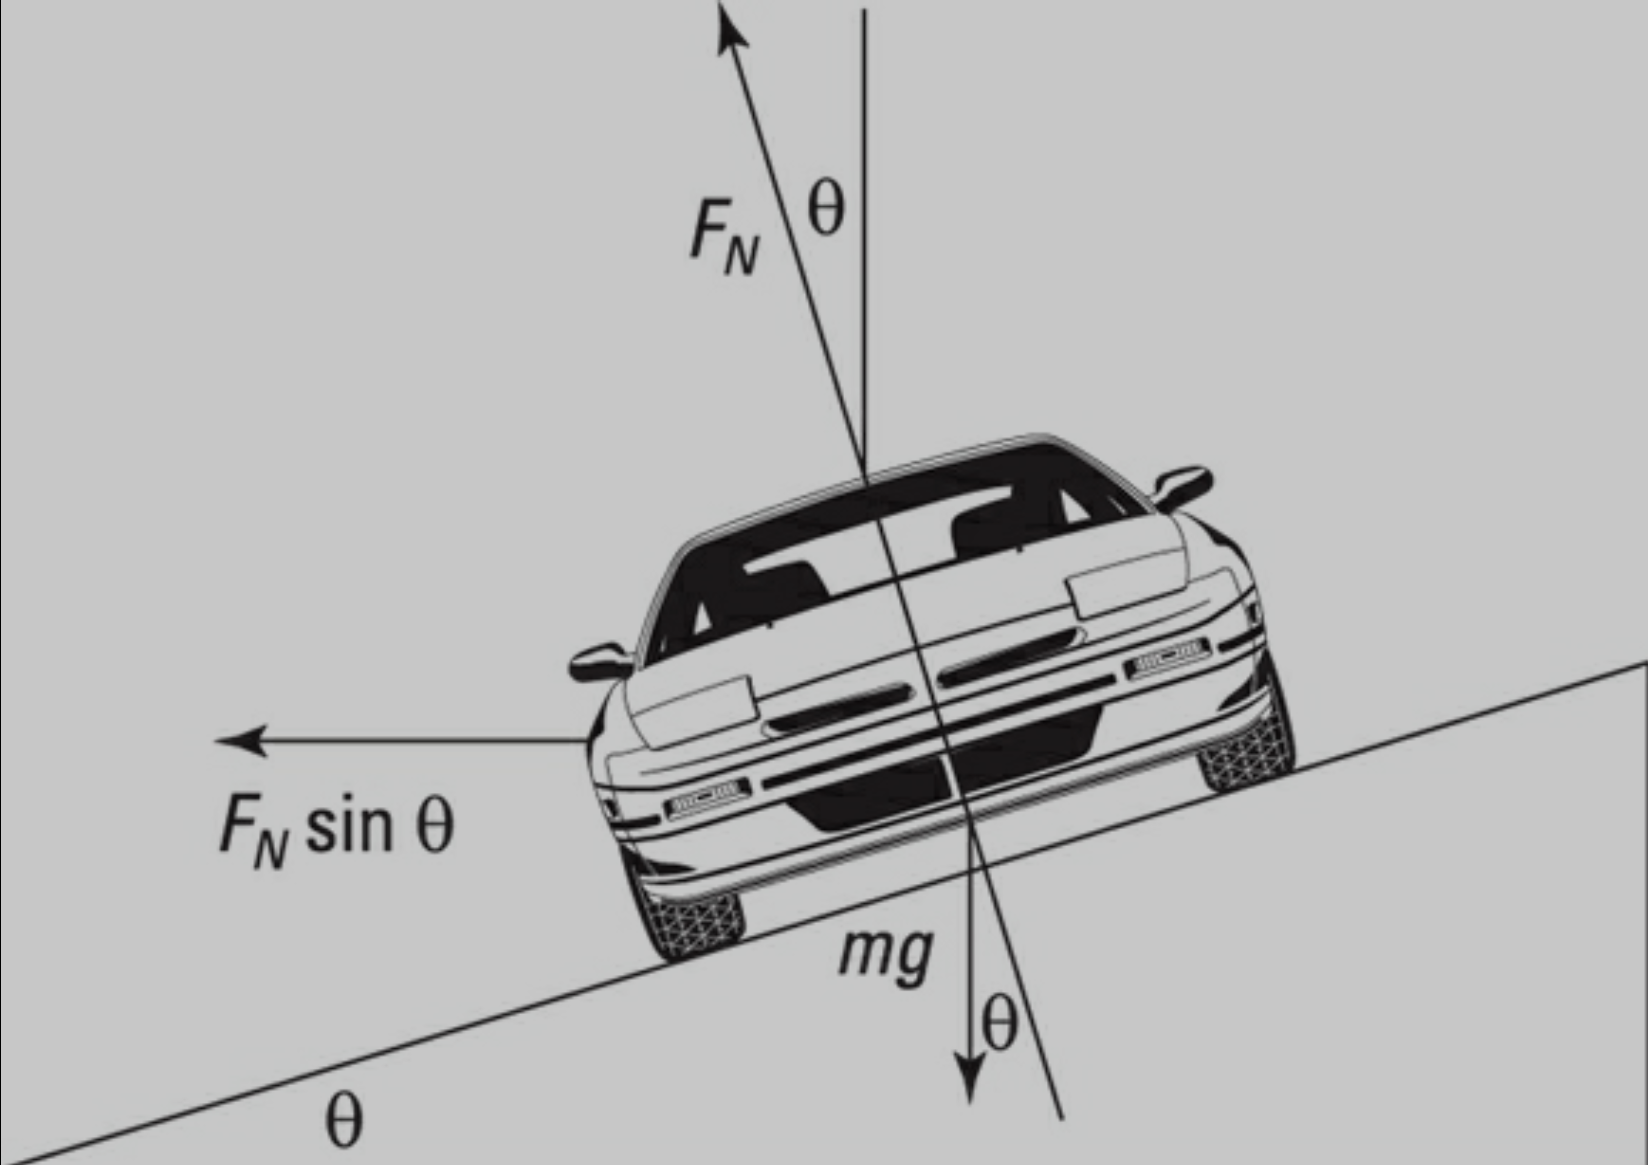
\includegraphics[width=\columnwidth]{image}
\\\\
Holzner, Steven. Physics I For Dummies (For Dummies (Math \& Science)) (p. 124). Wiley. Kindle Edition.
\\\\
\section{Solution}
\[ a_c=\frac{v^2}{r} \]
\[ F_N\sin(\theta)=F_c=\frac{mv^2}{R} \]
\[ F_N\cos(\theta)=mg \]
\[ \frac{mg}{\cos(\theta)}(\sin(\theta))=\frac{mv^2}{R} \]
\[ \frac{\sin(\theta)}{\cos(\theta)}=\tan(\theta) \]
\[ mg\tan(\theta)=\frac{mv^2}{R} \]
\[ \tan^{-1}=\frac{v^2}{gR} \]
\end{document}
